\chapter{Discussion}

If we focus on Android apps what are the implications and how relevant are the approaches and results? Apps are a popular and relevant subset of all software,they run remotely on other people’s equipment where they are the primary owners of the data on their devices, and where the platform and pre-installed platform software determine various aspects of the data collection

\section{Threats to Validity}
Using ratings and reviews to measure quality?

\section{Quis custodiet ipsos custodes?}
\url{https://en.wikipedia.org/wiki/Quis_custodiet_ipsos_custodes%3F}
Who watches the watchers? The app store is all powerful, promoting one app, demoting or even blocking another. What it reports is expected to be taken on trust. And who has time or resources to check or verify the veracity of what is being reported and to whom? 

\section{Android Vitals}
\subsection{Which apps can Android Vitals help?}
As Google only provides various reports in Android Vitals once they decide enough data exists to preserve the privacy of end users Android Vitals provides little for developers of less popular apps. 

Based on very rough approximations combining my case studies with AppBrain's download statistics to 19th June 2019, shown in figure \ref{fig:appbrain_download_statistics_jun_2019}\cite{appbrain_download_statistics_june_2019}, of the total populations of app developers:
\begin{itemize}
    \item 3\% to 4\% (those with 100,000 to 500,000 total downloads) will get limited value as at least one report will be provided.
    \item < 1\% (those with 500,000 to 1,000,000 total downloads) will get some value as many of the reports will be provided, but not all.
    \item 1\% (those with > 1,000,000 total downloads) will get extensive value as most/all the reports will be provided.
\end{itemize}

\begin{figure}
    \centering
    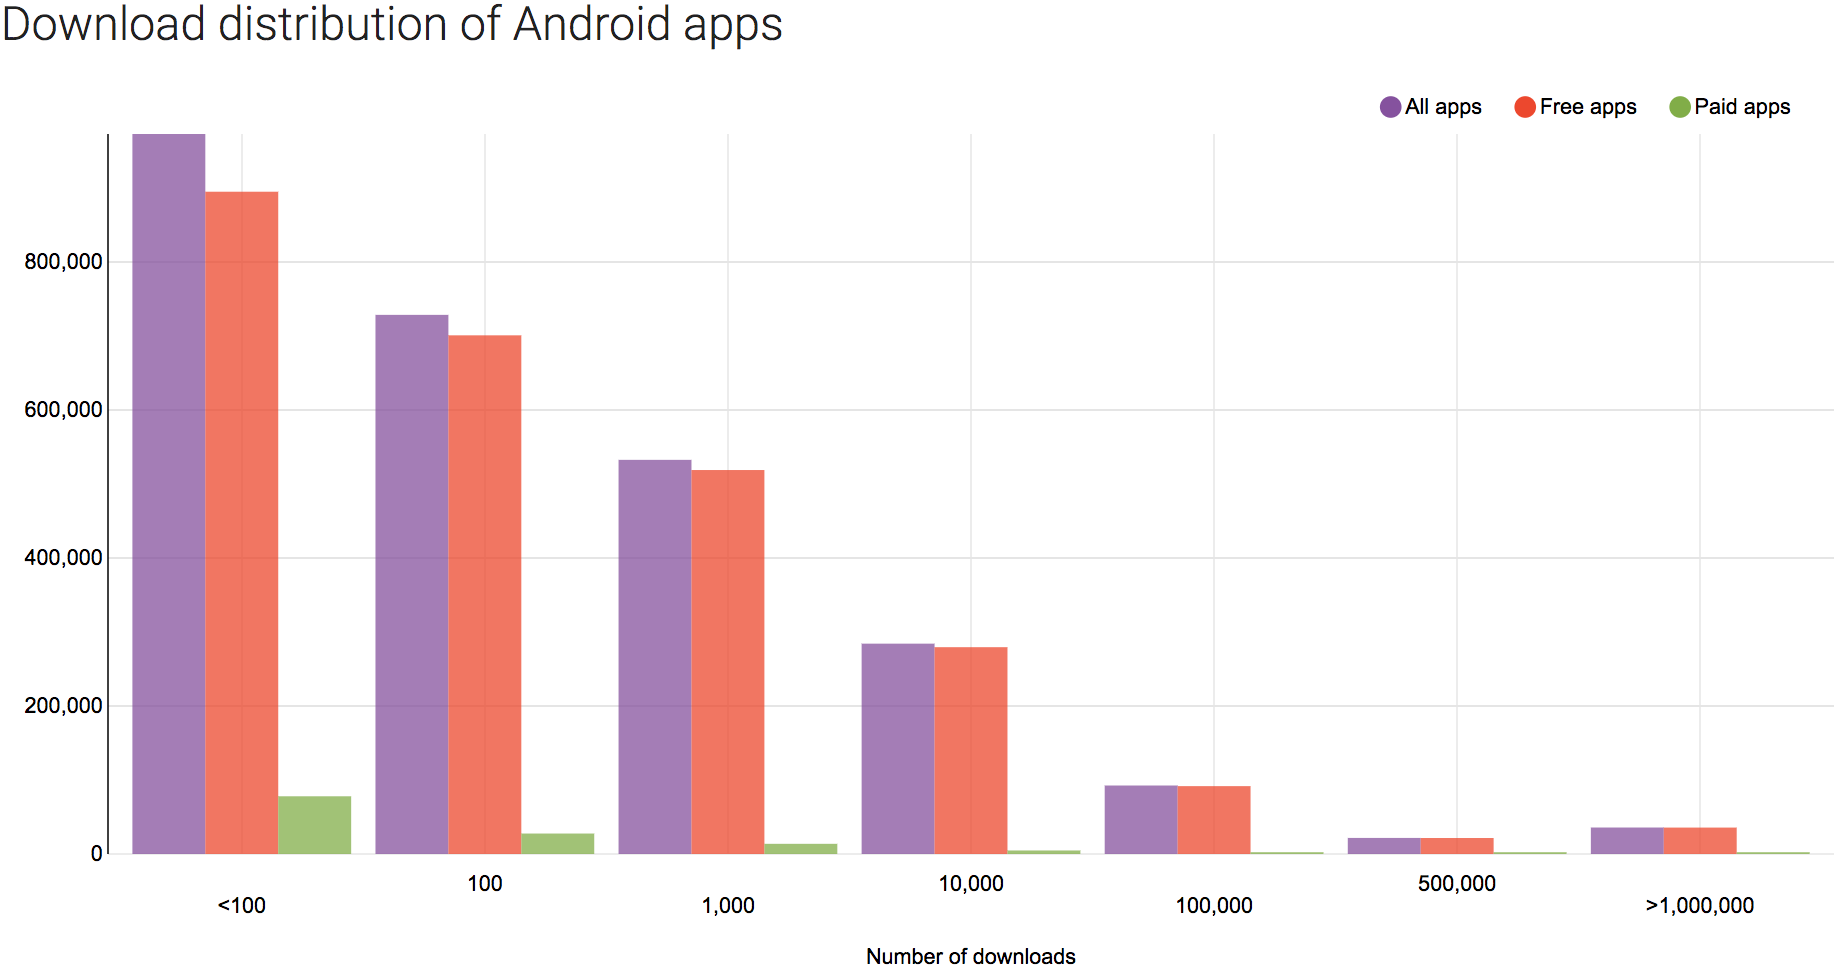
\includegraphics[width=\textwidth, keepaspectratio]{images/AppBrain_Download_Statistics_20-Jun-2019.png}
    \caption{AppBrain: Download distribution of Android apps (June 2019)}
    \label{fig:appbrain_download_statistics_jun_2019}
\end{figure}

\subsection{Who gets sufficient usage to see more detailed reports?}
Our limited insight into Android Vitals already indicates that reports are only provided when there is sufficient data collected to 'prime the pump'. It may be possible to estimate how many apps of those in Google Play Store are likely to have enough volumes of usage data. Google makes various recommendations for developers on how to apply the results Android Vitals reports \url{https://developer.android.com/distribute/best-practices/develop/android-vitals} however the developers can't do much until Android Vitals actually shows them the data. For apps with less than about 50k active installs \textit{("Installs on Active Devices (devices online in the past 30 days with this app installed)}." according to Google Play Console's tool tip). These counts are around 20\% to 30\% of the total install count for various apps used in our research \textit{e.g.} the active installs would be around 20k for an app that shows at having 100,000+ [total] installs to end users in Google Play.

Data provided by AppBrain\cite{appbrain_download_statistics_june_2019} was used to estimate the populations of apps that are not likely to generate enough data to see various reports in Android Vitals.
% wikimedes 5373 active installs - Crash rate by app version only (not device or Android version).
% wikimedzh 3769 active installs - no Android Vitals reports
% wikimedfa 2807 active installs - no Android Vitals reports
% 
Based on Android Vitals reports for Kiwix custom apps we infer that few apps with less than 20,000 total installs will have any detailed reports; WikiMed in Spanish has 5,373 active installs and has one report, for crash rate by app version. None of the other reports are available for this app. The threshold for when there is enough data for Google to provide a report depends on various factors, so the total installs is a proxy measurement and imperfect. Therefore Android Vitals is unlikely to offer much value for developers of (973,381 + 730,419 + 553,261 + 284,634) apps i.e. 2,541,695 apps in Google Play. For the next 92,678 the value of Android Vitals might increase somewhat, depending on how their app behaves and their user-base (e.g. are they on a few Android versions or spread across a spectrum - the larger the spread the less likely the reports will have data). And so on. By my admittedly limited view into the overall data set, Android Vitals is best placed to help the developers of the top (21,728 + 35,854) 57,582 apps, approximately 2\% to 3\% of the total population (2,691,955 apps). These apps (according to AppBrain's data on library use) are also more likely to use Firebase, Crashlytics, etc. so also have some of the run-time data available from these sources in addition to Android Vitals.

My work is to investigate two broad sources of data - data collected by the operating system (here effectively what appears in Android Vitals) and data collected using in-app libraries, particularly mobile analytics, it could include heatmapping (e.g. Appsee who you mention), crash handlers, etc. to provide feedback to measure how well the development team did in terms of testing and code quality. What they learn could also be useful to help them improve how they develop and test their apps in future, particularly with the greater detail mobile analytics (particularly Firebase) can provide the team.

\subsection{All that glitters is not gold}
Android Vitals sometimes reports excessive network usage running in the background while the device is running on battery, as shown in figure \ref{fig:android_vitals_excessive_network_usage}. As the Kiwix app is designed to enable users to download sometimes extremely large files, and to do so in the background, this warning is to be expected and not a bug - it's a feature. So, not everything that Android Vitals flags necessarily needs to be acted on. 
\begin{figure}
    \centering
    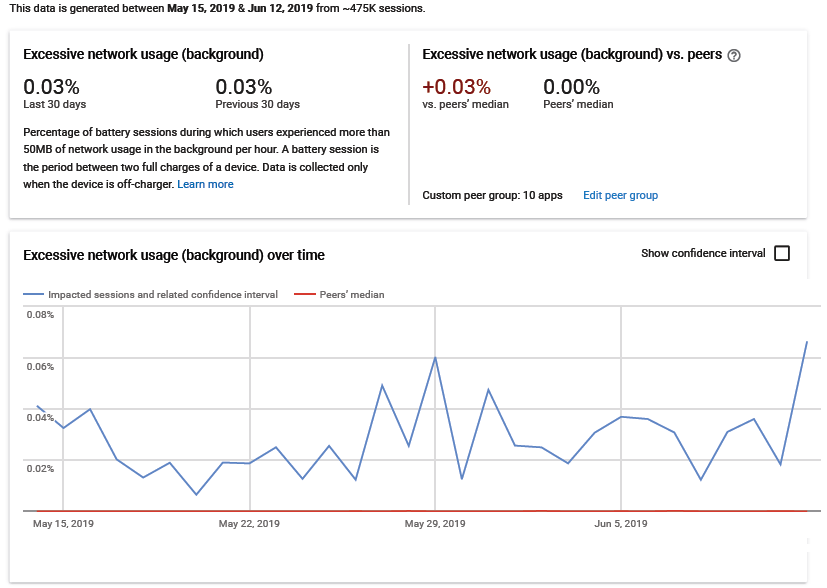
\includegraphics[width=\textwidth, keepaspectratio]{images/Excessive_network_usage_by_kiwix_15_jun_2019.png}
    \caption{Excessive background network usage on battery}
    \label{fig:android_vitals_excessive_network_usage}
\end{figure}

\section{Ethics of incorporating mobile analytics}
Tradeoffs; comparing other approaches which may have similar effect with less/no tracking.

Practical options:
\begin{itemize}
    \item Do as others do?
    \item Proportionate exchange of value: users do not pay for the app, and few actively provide feedback. Organ donation is far more intrusive and yet English law is changing\footnote{\url{https://www.organdonation.nhs.uk/uk-laws/}} to presume consent\cite{NHS_organ_donation_in_england} 
    \item Offer an opt-out
    \item Offer an opt-in
    \item leave the user to take action to provide information c.f. Kiwix-Android and Android Daisy Reader.
\end{itemize}

\subsection{Legal aspects of using mobile analytics for development and testing}

\begin{itemize}
    \item GDPR?
    \item PII vs non-PII information.
\end{itemize}

Data ownership and safeguarding.

Considerations and concerns when using Mobile Analytics
\begin{itemize}
    \item Privacy:
    \item Costs: financial, data, privacy, performance, bloat:
    \item Who owns the data and who gets to use it?:
    \item Stewardship: Impact(s) of having access to sensitive and valuable data.
    \item Performance:
    \item Sufficiency: is the data we collect sufficient to enable us to achieve our objectives of improving testing.
\end{itemize}


\subsection{Necessary? Sufficient?}
Freezes and crashes may adversely impact a user's perspective, Google may limit the visibility of apps that score poorly in terms of 'stability' as I will cover later in my thesis. However, are performant applications sufficient to thrive? There may be other barriers, or hurdles, developers need to overcome such as providing software that is attractive, serves whatever the user wants to do, and is intuitive.

In 2019 Menzies in his paper \emph{``Take Control: On the Unreasonable Effectiveness of Software Analytics"}~\cite{menzies2019take} indicates that a small number of predictable software analytics variables can be used to predict software qualities for projects. 

\emph{``Specifically, the number of variables required to make predictions about SE projects is remarkably small which means that (a) most of the things we think might affect software quality have little impact in practice; (b) controlling just a few key variables can be enough to improve software quality."}

\subsubsection{Validity from the Google Engineering Team}

MUST\_DO Use the beyond Google Play paper to help support the validity of my research.

\subsubsection{Other Android App Stores?}
Note: this research is limited to apps available in Google Play for practical reasons. Other Android app stores are available, particularly in China as Wang ~\emph{et al} (2018)~\cite{wang2018beyond} describes. Of the Chinese app stores, in 2018 only 2 (Tencent Myapp, and 360 Market) provided a quality rating. In email discussions of my research in 2020 one of that paper's authors, Li Li, confirmed the novelty, importance and relevance of my research.